% Side experiments P1 (memory depth) and P2 (item intercept), added 2026-09-19.
% Plan: claude/side_experiments_plan_2026-09-19.md. Results archive: docs/experiments/paper_side_experiments_results.md.
% The figure is generated by tools/build_figs.py from evidence/numbers.yaml; the ids behind every mark are in figs/_fig_report.json.
% 2026-09-20: the former Figures 2 and 3 were merged into one three-panel figure, and the
% reading rules that stood in their captions moved into the Setup and Findings text.
\subsection{What the Memory State Carries}
\label{sec:exp_memory}

\textbf{Question.} RQ1c, in two parts: how many past readings the state needs, and whether the gain from memory is inter-turn dynamics or a fixed level per prompt item.
\textbf{Setup.} Tasks, baselines and the skill score follow \S\ref{sec:exp_setup}; both experiments vary one thing in the KOMPAS (linear) row of Table~\ref{tab:prediction}.
Table~\ref{tab:prediction} fits each row on every transition its state can be formed from, so a one-reading state trains on earlier turns than a four-reading state.  % paper_side_experiments_results.md section 1.2, default caliber
Both experiments here fit every depth on the same set of transitions, which separates the depth of the state from the size of its training set.  % matched caliber; figs/_fig_report.json
Under that matched window the memory gain on sentence length shrinks from +0.603 in Table~\ref{tab:prediction} to +0.109, so the two calibers answer different questions.  % n_main_013 (default) vs n_abl_127 (matched)
In every panel of Figure~\ref{fig:memory} a filled marker means the 95\% paired bootstrap interval excludes zero, and a hollow marker means it contains zero.  % moved out of the former Figure 2 and Figure 3 captions, 2026-09-20

\begin{figure}[t]
\centering
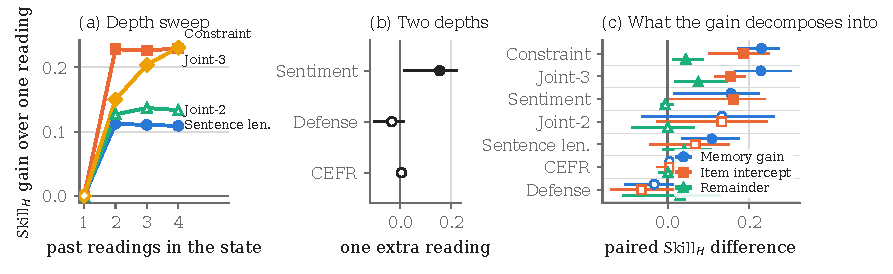
\includegraphics[width=\linewidth]{figs/fig_memory.pdf}
\caption{How deep the memory state has to be, and what its gain decomposes into, both under a matched training window. (a) Gain of a state holding $d$ past readings over a state holding one, on the four tasks whose design allows a sweep. (b) The same gain for one extra reading on the three designs that carry two depths. (c) Three paired differences per task of Table~\ref{tab:prediction}.}
\label{fig:memory}
\end{figure}

\textbf{Findings, depth.} On three of the four sweepable tasks the second reading buys the whole gain: +0.112 on sentence length, +0.228 on Joint-3, +0.127 on Joint-2.  % c10; n_abl_124 n_abl_184 n_abl_157
The third and fourth readings add no more than 0.010 on those three tasks.  % n_abl_126 n_abl_128 n_abl_186 n_abl_188 n_abl_159 n_abl_161
The Joint-2 interval contains zero at every depth.  % n_abl_157 n_abl_158 n_abl_160
Constraint is the exception: each added turn keeps paying, +0.149, +0.054 and +0.027 for the second, third and fourth, each with an interval excluding zero.  % n_abl_235 n_abl_237 n_abl_239
Of the three two-depth tasks, sentiment gains +0.155 from one extra reading, while defense and CEFR do not separate from zero.  % n_abl_151 (caveated: two cells) n_abl_245 n_abl_262
The driver is that a level and a trend take two readings to express, and the attribute tasks carry little structure beyond that pair.  % m1
No mechanism is established for why constraint keeps gaining, and none is proposed here.  % c10 notes

\textbf{Findings, item intercept.} Panel (c) carries three paired differences per task: the memory gain over Last-turn, the part an added per-item intercept recovers, and what remains beyond that intercept.  % moved out of the former Figure 3 caption
Intercepts are estimated on turns outside the scored window.  % moved out of the former Figure 3 caption
A per-item intercept added to the one-reading state recovers most of the memory gain: 81\% on constraint and 67\% on Joint-3.  % c11; n_mech_061/n_mech_060=0.807, n_mech_058/n_mech_057=0.673
What remains after the intercept is +0.045 on constraint and +0.075 on Joint-3, both with intervals excluding zero.  % n_mech_059 n_mech_056
On the other five tasks the remainder does not separate from zero, and on sentiment and Joint-2 the intercept accounts for the whole gain.  % n_mech_050 n_mech_053 n_mech_047 n_mech_068 n_mech_062; n_mech_052 vs n_mech_051, n_mech_055 vs n_mech_054
The driver is that each prompt item holds its own level across turns, and several past readings estimate that level where one reading cannot.  % m6
Inter-turn dynamics beyond that level is measured on two tasks, and it is the smaller of the two parts on both.  % c11 notes

Together, \uline{one extra reading carries most of what memory buys, and most of that is a per-item level rather than inter-turn dynamics; this answers RQ1c. A remainder attributable to dynamics is measured on two of seven tasks.}
